\documentclass[1p]{elsarticle_modified}
%\bibliographystyle{elsarticle-num}

%\usepackage[colorlinks]{hyperref}
%\usepackage{abbrmath_seonhwa} %\Abb, \Ascr, \Acal ,\Abf, \Afrak
\usepackage{amsfonts}
\usepackage{amssymb}
\usepackage{amsmath}
\usepackage{amsthm}
\usepackage{scalefnt}
\usepackage{amsbsy}
\usepackage{kotex}
\usepackage{caption}
\usepackage{subfig}
\usepackage{color}
\usepackage{graphicx}
\usepackage{xcolor} %% white, black, red, green, blue, cyan, magenta, yellow
\usepackage{float}
\usepackage{setspace}
\usepackage{hyperref}

\usepackage{tikz}
\usetikzlibrary{arrows}

\usepackage{multirow}
\usepackage{array} % fixed length table
\usepackage{hhline}

%%%%%%%%%%%%%%%%%%%%%
\makeatletter
\renewcommand*\env@matrix[1][\arraystretch]{%
	\edef\arraystretch{#1}%
	\hskip -\arraycolsep
	\let\@ifnextchar\new@ifnextchar
	\array{*\c@MaxMatrixCols c}}
\makeatother %https://tex.stackexchange.com/questions/14071/how-can-i-increase-the-line-spacing-in-a-matrix
%%%%%%%%%%%%%%%

\usepackage[normalem]{ulem}

\newcommand{\msout}[1]{\ifmmode\text{\sout{\ensuremath{#1}}}\else\sout{#1}\fi}
%SOURCE: \msout is \stkout macro in https://tex.stackexchange.com/questions/20609/strikeout-in-math-mode

\newcommand{\cancel}[1]{
	\ifmmode
	{\color{red}\msout{#1}}
	\else
	{\color{red}\sout{#1}}
	\fi
}

\newcommand{\add}[1]{
	{\color{blue}\uwave{#1}}
}

\newcommand{\replace}[2]{
	\ifmmode
	{\color{red}\msout{#1}}{\color{blue}\uwave{#2}}
	\else
	{\color{red}\sout{#1}}{\color{blue}\uwave{#2}}
	\fi
}

\newcommand{\Sol}{\mathcal{S}} %segment
\newcommand{\D}{D} %diagram
\newcommand{\A}{\mathcal{A}} %arc


%%%%%%%%%%%%%%%%%%%%%%%%%%%%%5 test

\def\sl{\operatorname{\textup{SL}}(2,\Cbb)}
\def\psl{\operatorname{\textup{PSL}}(2,\Cbb)}
\def\quan{\mkern 1mu \triangleright \mkern 1mu}

\theoremstyle{definition}
\newtheorem{thm}{Theorem}[section]
\newtheorem{prop}[thm]{Proposition}
\newtheorem{lem}[thm]{Lemma}
\newtheorem{ques}[thm]{Question}
\newtheorem{cor}[thm]{Corollary}
\newtheorem{defn}[thm]{Definition}
\newtheorem{exam}[thm]{Example}
\newtheorem{rmk}[thm]{Remark}
\newtheorem{alg}[thm]{Algorithm}

\newcommand{\I}{\sqrt{-1}}
\begin{document}

%\begin{frontmatter}
%
%\title{Boundary parabolic representations of knots up to 8 crossings}
%
%%% Group authors per affiliation:
%\author{Yunhi Cho} 
%\address{Department of Mathematics, University of Seoul, Seoul, Korea}
%\ead{yhcho@uos.ac.kr}
%
%
%\author{Seonhwa Kim} %\fnref{s_kim}}
%\address{Center for Geometry and Physics, Institute for Basic Science, Pohang, 37673, Korea}
%\ead{ryeona17@ibs.re.kr}
%
%\author{Hyuk Kim}
%\address{Department of Mathematical Sciences, Seoul National University, Seoul 08826, Korea}
%\ead{hyukkim@snu.ac.kr}
%
%\author{Seokbeom Yoon}
%\address{Department of Mathematical Sciences, Seoul National University, Seoul, 08826,  Korea}
%\ead{sbyoon15@snu.ac.kr}
%
%\begin{abstract}
%We find all boundary parabolic representation of knots up to 8 crossings.
%
%\end{abstract}
%\begin{keyword}
%    \MSC[2010] 57M25 
%\end{keyword}
%
%\end{frontmatter}

%\linenumbers
%\tableofcontents
%
\newcommand\colored[1]{\textcolor{white}{\rule[-0.35ex]{0.8em}{1.4ex}}\kern-0.8em\color{red} #1}%
%\newcommand\colored[1]{\textcolor{white}{ #1}\kern-2.17ex	\textcolor{white}{ #1}\kern-1.81ex	\textcolor{white}{ #1}\kern-2.15ex\color{red}#1	}

{\Large $\underline{11a_{267}~(K11a_{267})}$}

\setlength{\tabcolsep}{10pt}
\renewcommand{\arraystretch}{1.6}
\vspace{1cm}\begin{tabular}{m{100pt}>{\centering\arraybackslash}m{274pt}}
\multirow{5}{120pt}{
	\centering
	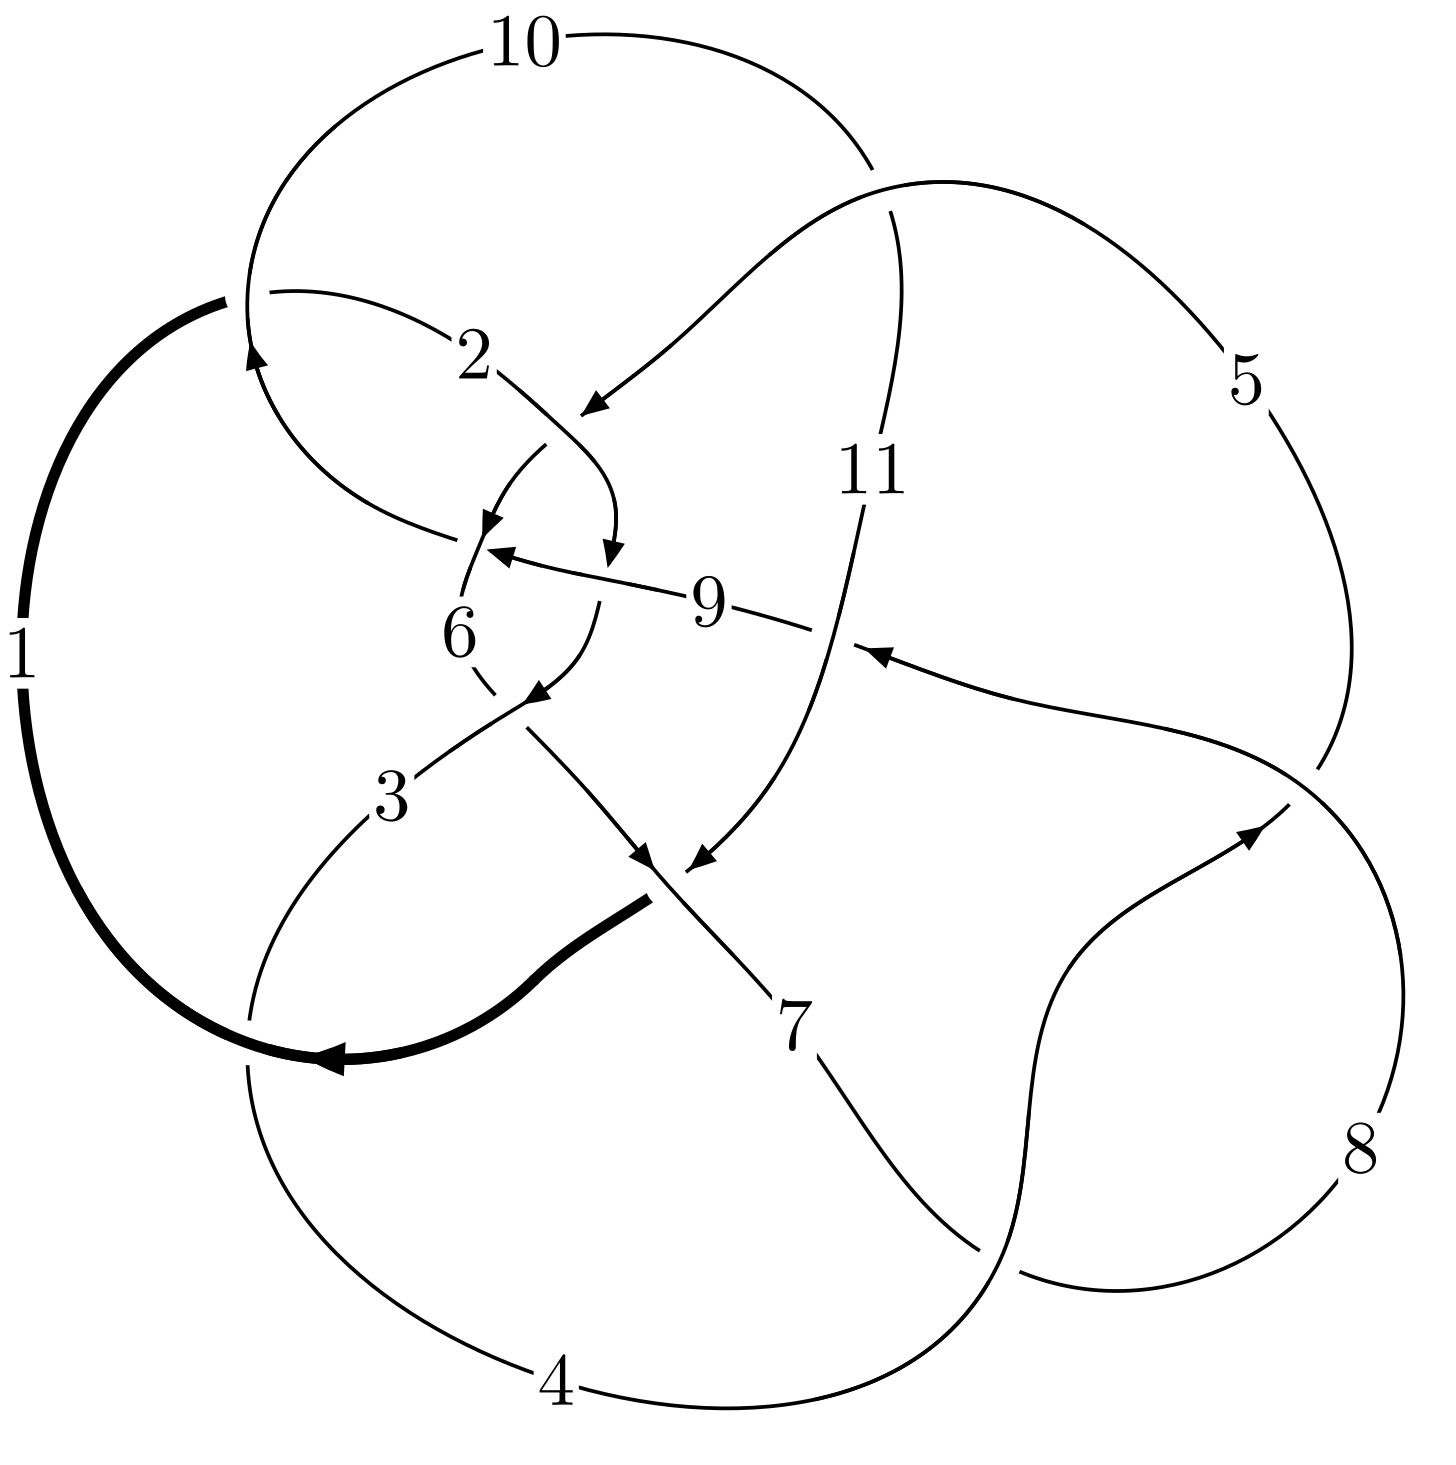
\includegraphics[width=112pt]{../../../GIT/diagram.site/Diagrams/png/516_11a_267.png}\\
\ \ \ A knot diagram\footnotemark}&
\allowdisplaybreaks
\textbf{Linearized knot diagam} \\
\cline{2-2}
 &
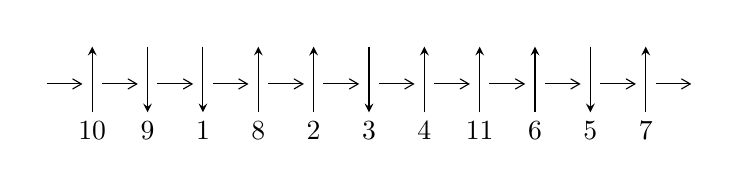
\begin{tikzpicture}[x=20pt, y=17pt]
	% nodes
	\node (C0) at (0, 0) {};
	\node (C1) at (1, 0) {};
	\node (C1U) at (1, +1) {};
	\node (C1D) at (1, -1) {10};

	\node (C2) at (2, 0) {};
	\node (C2U) at (2, +1) {};
	\node (C2D) at (2, -1) {9};

	\node (C3) at (3, 0) {};
	\node (C3U) at (3, +1) {};
	\node (C3D) at (3, -1) {1};

	\node (C4) at (4, 0) {};
	\node (C4U) at (4, +1) {};
	\node (C4D) at (4, -1) {8};

	\node (C5) at (5, 0) {};
	\node (C5U) at (5, +1) {};
	\node (C5D) at (5, -1) {2};

	\node (C6) at (6, 0) {};
	\node (C6U) at (6, +1) {};
	\node (C6D) at (6, -1) {3};

	\node (C7) at (7, 0) {};
	\node (C7U) at (7, +1) {};
	\node (C7D) at (7, -1) {4};

	\node (C8) at (8, 0) {};
	\node (C8U) at (8, +1) {};
	\node (C8D) at (8, -1) {11};

	\node (C9) at (9, 0) {};
	\node (C9U) at (9, +1) {};
	\node (C9D) at (9, -1) {6};

	\node (C10) at (10, 0) {};
	\node (C10U) at (10, +1) {};
	\node (C10D) at (10, -1) {5};

	\node (C11) at (11, 0) {};
	\node (C11U) at (11, +1) {};
	\node (C11D) at (11, -1) {7};
	\node (C12) at (12, 0) {};

	% arrows
	\draw[->,>={angle 60}]
	(C0) edge (C1) (C1) edge (C2) (C2) edge (C3) (C3) edge (C4) (C4) edge (C5) (C5) edge (C6) (C6) edge (C7) (C7) edge (C8) (C8) edge (C9) (C9) edge (C10) (C10) edge (C11) (C11) edge (C12) ;	\draw[->,>=stealth]
	(C1D) edge (C1U) (C2U) edge (C2D) (C3U) edge (C3D) (C4D) edge (C4U) (C5D) edge (C5U) (C6U) edge (C6D) (C7D) edge (C7U) (C8D) edge (C8U) (C9D) edge (C9U) (C10U) edge (C10D) (C11D) edge (C11U) ;
	\end{tikzpicture} \\
\hhline{~~} \\& 
\textbf{Solving Sequence} \\ \cline{2-2} 
 &
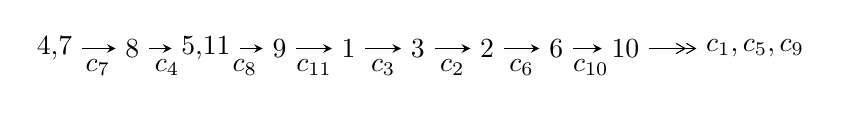
\begin{tikzpicture}[x=25pt, y=7pt]
	% node
	\node (A0) at (-1/8, 0) {4,7};
	\node (A1) at (1, 0) {8};
	\node (A2) at (33/16, 0) {5,11};
	\node (A3) at (25/8, 0) {9};
	\node (A4) at (33/8, 0) {1};
	\node (A5) at (41/8, 0) {3};
	\node (A6) at (49/8, 0) {2};
	\node (A7) at (57/8, 0) {6};
	\node (A8) at (65/8, 0) {10};
	\node (C1) at (1/2, -1) {$c_{7}$};
	\node (C2) at (3/2, -1) {$c_{4}$};
	\node (C3) at (21/8, -1) {$c_{8}$};
	\node (C4) at (29/8, -1) {$c_{11}$};
	\node (C5) at (37/8, -1) {$c_{3}$};
	\node (C6) at (45/8, -1) {$c_{2}$};
	\node (C7) at (53/8, -1) {$c_{6}$};
	\node (C8) at (61/8, -1) {$c_{10}$};
	\node (A9) at (10, 0) {$c_{1},c_{5},c_{9}$};

	% edge
	\draw[->,>=stealth]	
	(A0) edge (A1) (A1) edge (A2) (A2) edge (A3) (A3) edge (A4) (A4) edge (A5) (A5) edge (A6) (A6) edge (A7) (A7) edge (A8) ;
	\draw[->>,>={angle 60}]	
	(A8) edge (A9);
\end{tikzpicture} \\ 

\end{tabular} \\

\footnotetext{
The image of knot diagram is generated by the software ``\textbf{Draw programme}" developed by Andrew Bartholomew(\url{http://www.layer8.co.uk/maths/draw/index.htm\#Running-draw}), where we modified some parts for our purpose(\url{https://github.com/CATsTAILs/LinksPainter}).
}\phantom \\ \newline 
\centering \textbf{Ideals for irreducible components\footnotemark of $X_{\text{par}}$} 
 
\begin{align*}
I^u_{1}&=\langle 
3.44670\times10^{407} u^{114}-8.42803\times10^{407} u^{113}+\cdots+1.19387\times10^{407} b-2.77971\times10^{408},\\
\phantom{I^u_{1}}&\phantom{= \langle  }-9.47292\times10^{408} u^{114}+2.83965\times10^{409} u^{113}+\cdots+3.70100\times10^{408} a-2.62544\times10^{410},\\
\phantom{I^u_{1}}&\phantom{= \langle  }u^{115}- u^{114}+\cdots-541 u-31\rangle \\
I^u_{2}&=\langle 
-861785 u^{19}-14841113 u^{18}+\cdots+21120991 b+29316743,\\
\phantom{I^u_{2}}&\phantom{= \langle  }17202656 u^{19}+68033143 u^{18}+\cdots+21120991 a-84886177,\;u^{20}+2 u^{19}+\cdots+9 u-1\rangle \\
\\
\end{align*}
\raggedright * 2 irreducible components of $\dim_{\mathbb{C}}=0$, with total 135 representations.\\
\footnotetext{All coefficients of polynomials are rational numbers. But the coefficients are sometimes approximated in decimal forms when there is not enough margin.}
\newpage
\renewcommand{\arraystretch}{1}
\centering \section*{I. $I^u_{1}= \langle 3.45\times10^{407} u^{114}-8.43\times10^{407} u^{113}+\cdots+1.19\times10^{407} b-2.78\times10^{408},\;-9.47\times10^{408} u^{114}+2.84\times10^{409} u^{113}+\cdots+3.70\times10^{408} a-2.63\times10^{410},\;u^{115}- u^{114}+\cdots-541 u-31 \rangle$}
\flushleft \textbf{(i) Arc colorings}\\
\begin{tabular}{m{7pt} m{180pt} m{7pt} m{180pt} }
\flushright $a_{4}=$&$\begin{pmatrix}0\\u\end{pmatrix}$ \\
\flushright $a_{7}=$&$\begin{pmatrix}1\\0\end{pmatrix}$ \\
\flushright $a_{8}=$&$\begin{pmatrix}1\\- u^2\end{pmatrix}$ \\
\flushright $a_{5}=$&$\begin{pmatrix}u\\- u^3+u\end{pmatrix}$ \\
\flushright $a_{11}=$&$\begin{pmatrix}2.55956 u^{114}-7.67264 u^{113}+\cdots+860.734 u+70.9387\\-2.88700 u^{114}+7.05941 u^{113}+\cdots+545.327 u+23.2831\end{pmatrix}$ \\
\flushright $a_{9}=$&$\begin{pmatrix}1.35442 u^{114}-4.78591 u^{113}+\cdots+1006.67 u+76.1821\\-0.574110 u^{114}+2.15598 u^{113}+\cdots-667.441 u-53.4608\end{pmatrix}$ \\
\flushright $a_{1}=$&$\begin{pmatrix}-0.327442 u^{114}-0.613229 u^{113}+\cdots+1406.06 u+94.2218\\-2.88700 u^{114}+7.05941 u^{113}+\cdots+545.327 u+23.2831\end{pmatrix}$ \\
\flushright $a_{3}=$&$\begin{pmatrix}0.149706 u^{114}-0.860592 u^{113}+\cdots+314.269 u+19.5982\\-3.86467 u^{114}+7.94980 u^{113}+\cdots+2027.33 u+124.487\end{pmatrix}$ \\
\flushright $a_{2}=$&$\begin{pmatrix}-0.639730 u^{114}+0.865923 u^{113}+\cdots+690.842 u+40.8469\\-3.05087 u^{114}+5.84910 u^{113}+\cdots+2187.57 u+143.045\end{pmatrix}$ \\
\flushright $a_{6}=$&$\begin{pmatrix}-0.745287 u^{114}+0.449774 u^{113}+\cdots+1257.74 u+86.8139\\1.57302 u^{114}-3.23099 u^{113}+\cdots-751.386 u-45.9144\end{pmatrix}$ \\
\flushright $a_{10}=$&$\begin{pmatrix}0.183301 u^{114}-1.96737 u^{113}+\cdots+1494.73 u+104.855\\-1.12054 u^{114}+3.53741 u^{113}+\cdots-548.015 u-45.9997\end{pmatrix}$\\ \flushright $a_{10}=$&$\begin{pmatrix}0.183301 u^{114}-1.96737 u^{113}+\cdots+1494.73 u+104.855\\-1.12054 u^{114}+3.53741 u^{113}+\cdots-548.015 u-45.9997\end{pmatrix}$\\&\end{tabular}
\flushleft \textbf{(ii) Obstruction class $= -1$}\\~\\
\flushleft \textbf{(iii) Cusp Shapes $= -21.2534 u^{114}+34.5236 u^{113}+\cdots+23037.7 u+1611.82$}\\~\\
\newpage\renewcommand{\arraystretch}{1}
\flushleft \textbf{(iv) u-Polynomials at the component}\newline \\
\begin{tabular}{m{50pt}|m{274pt}}
Crossings & \hspace{64pt}u-Polynomials at each crossing \\
\hline $$\begin{aligned}c_{1}\end{aligned}$$&$\begin{aligned}
&u^{115}-5 u^{114}+\cdots-30 u-1
\end{aligned}$\\
\hline $$\begin{aligned}c_{2}\end{aligned}$$&$\begin{aligned}
&u^{115}- u^{114}+\cdots+34 u-1
\end{aligned}$\\
\hline $$\begin{aligned}c_{3}\end{aligned}$$&$\begin{aligned}
&u^{115}+u^{114}+\cdots-138 u+23
\end{aligned}$\\
\hline $$\begin{aligned}c_{4},c_{7}\end{aligned}$$&$\begin{aligned}
&u^{115}+u^{114}+\cdots-541 u+31
\end{aligned}$\\
\hline $$\begin{aligned}c_{5}\end{aligned}$$&$\begin{aligned}
&u^{115}-5 u^{114}+\cdots-11 u+1
\end{aligned}$\\
\hline $$\begin{aligned}c_{6}\end{aligned}$$&$\begin{aligned}
&u^{115}- u^{114}+\cdots+48 u-1
\end{aligned}$\\
\hline $$\begin{aligned}c_{8}\end{aligned}$$&$\begin{aligned}
&u^{115}-3 u^{114}+\cdots-3684 u+691
\end{aligned}$\\
\hline $$\begin{aligned}c_{9}\end{aligned}$$&$\begin{aligned}
&u^{115}-7 u^{114}+\cdots+2 u+1
\end{aligned}$\\
\hline $$\begin{aligned}c_{10}\end{aligned}$$&$\begin{aligned}
&u^{115}- u^{114}+\cdots+668365 u-39479
\end{aligned}$\\
\hline $$\begin{aligned}c_{11}\end{aligned}$$&$\begin{aligned}
&u^{115}+u^{114}+\cdots-5 u+1
\end{aligned}$\\
\hline
\end{tabular}\\~\\
\newpage\renewcommand{\arraystretch}{1}
\flushleft \textbf{(v) Riley Polynomials at the component}\newline \\
\begin{tabular}{m{50pt}|m{274pt}}
Crossings & \hspace{64pt}Riley Polynomials at each crossing \\
\hline $$\begin{aligned}c_{1}\end{aligned}$$&$\begin{aligned}
&y^{115}-15 y^{114}+\cdots-10 y-1
\end{aligned}$\\
\hline $$\begin{aligned}c_{2}\end{aligned}$$&$\begin{aligned}
&y^{115}-9 y^{114}+\cdots+20 y-1
\end{aligned}$\\
\hline $$\begin{aligned}c_{3}\end{aligned}$$&$\begin{aligned}
&y^{115}+13 y^{114}+\cdots+2346 y-529
\end{aligned}$\\
\hline $$\begin{aligned}c_{4},c_{7}\end{aligned}$$&$\begin{aligned}
&y^{115}-87 y^{114}+\cdots+12627 y-961
\end{aligned}$\\
\hline $$\begin{aligned}c_{5}\end{aligned}$$&$\begin{aligned}
&y^{115}-3 y^{114}+\cdots+y-1
\end{aligned}$\\
\hline $$\begin{aligned}c_{6}\end{aligned}$$&$\begin{aligned}
&y^{115}-31 y^{114}+\cdots+416 y-1
\end{aligned}$\\
\hline $$\begin{aligned}c_{8}\end{aligned}$$&$\begin{aligned}
&y^{115}-31 y^{114}+\cdots+17763462 y-477481
\end{aligned}$\\
\hline $$\begin{aligned}c_{9}\end{aligned}$$&$\begin{aligned}
&y^{115}+15 y^{114}+\cdots+62 y-1
\end{aligned}$\\
\hline $$\begin{aligned}c_{10}\end{aligned}$$&$\begin{aligned}
&y^{115}+47 y^{114}+\cdots-11408069835 y-1558591441
\end{aligned}$\\
\hline $$\begin{aligned}c_{11}\end{aligned}$$&$\begin{aligned}
&y^{115}-11 y^{114}+\cdots+139 y-1
\end{aligned}$\\
\hline
\end{tabular}\\~\\
\newpage\flushleft \textbf{(vi) Complex Volumes and Cusp Shapes}
$$\begin{array}{c|c|c}  
\text{Solutions to }I^u_{1}& \I (\text{vol} + \sqrt{-1}CS) & \text{Cusp shape}\\
 \hline 
\begin{aligned}
u &= \phantom{-}0.991543 + 0.010287 I \\
a &= \phantom{-}0.508535 - 0.816617 I \\
b &= -0.337478 - 1.075160 I\end{aligned}
 & -0.82850 + 3.65420 I & \phantom{-0.000000 } 0 \\ \hline\begin{aligned}
u &= \phantom{-}0.991543 - 0.010287 I \\
a &= \phantom{-}0.508535 + 0.816617 I \\
b &= -0.337478 + 1.075160 I\end{aligned}
 & -0.82850 - 3.65420 I & \phantom{-0.000000 } 0 \\ \hline\begin{aligned}
u &= \phantom{-}0.812804 + 0.602814 I \\
a &= \phantom{-}0.505084 - 0.733259 I \\
b &= -0.095403 - 0.810136 I\end{aligned}
 & -2.33628 + 2.44376 I & \phantom{-0.000000 } 0 \\ \hline\begin{aligned}
u &= \phantom{-}0.812804 - 0.602814 I \\
a &= \phantom{-}0.505084 + 0.733259 I \\
b &= -0.095403 + 0.810136 I\end{aligned}
 & -2.33628 - 2.44376 I & \phantom{-0.000000 } 0 \\ \hline\begin{aligned}
u &= -0.957079 + 0.376972 I \\
a &= \phantom{-}1.019680 + 0.078149 I \\
b &= -0.996791 + 0.525819 I\end{aligned}
 & \phantom{-}1.93159 - 0.86279 I & \phantom{-0.000000 } 0 \\ \hline\begin{aligned}
u &= -0.957079 - 0.376972 I \\
a &= \phantom{-}1.019680 - 0.078149 I \\
b &= -0.996791 - 0.525819 I\end{aligned}
 & \phantom{-}1.93159 + 0.86279 I & \phantom{-0.000000 } 0 \\ \hline\begin{aligned}
u &= -0.866010 + 0.581201 I \\
a &= -0.748848 - 0.422099 I \\
b &= -0.1266320 - 0.0106676 I\end{aligned}
 & -0.17579 - 2.00781 I & \phantom{-0.000000 } 0 \\ \hline\begin{aligned}
u &= -0.866010 - 0.581201 I \\
a &= -0.748848 + 0.422099 I \\
b &= -0.1266320 + 0.0106676 I\end{aligned}
 & -0.17579 + 2.00781 I & \phantom{-0.000000 } 0 \\ \hline\begin{aligned}
u &= -1.009830 + 0.275630 I \\
a &= \phantom{-}2.55989 - 0.05597 I \\
b &= -0.110358 + 0.270869 I\end{aligned}
 & \phantom{-}1.03851 - 9.43459 I & \phantom{-0.000000 } 0 \\ \hline\begin{aligned}
u &= -1.009830 - 0.275630 I \\
a &= \phantom{-}2.55989 + 0.05597 I \\
b &= -0.110358 - 0.270869 I\end{aligned}
 & \phantom{-}1.03851 + 9.43459 I & \phantom{-0.000000 } 0\\
 \hline 
 \end{array}$$\newpage$$\begin{array}{c|c|c}  
\text{Solutions to }I^u_{1}& \I (\text{vol} + \sqrt{-1}CS) & \text{Cusp shape}\\
 \hline 
\begin{aligned}
u &= -0.654350 + 0.822893 I \\
a &= \phantom{-}0.039752 - 0.837771 I \\
b &= \phantom{-}0.364684 - 0.662893 I\end{aligned}
 & -1.04548 - 3.54916 I & \phantom{-0.000000 } 0 \\ \hline\begin{aligned}
u &= -0.654350 - 0.822893 I \\
a &= \phantom{-}0.039752 + 0.837771 I \\
b &= \phantom{-}0.364684 + 0.662893 I\end{aligned}
 & -1.04548 + 3.54916 I & \phantom{-0.000000 } 0 \\ \hline\begin{aligned}
u &= \phantom{-}0.854965 + 0.408531 I \\
a &= \phantom{-}1.37117 - 0.36061 I \\
b &= -0.088123 - 0.474534 I\end{aligned}
 & -2.08760 + 1.97298 I & \phantom{-0.000000 } 0 \\ \hline\begin{aligned}
u &= \phantom{-}0.854965 - 0.408531 I \\
a &= \phantom{-}1.37117 + 0.36061 I \\
b &= -0.088123 + 0.474534 I\end{aligned}
 & -2.08760 - 1.97298 I & \phantom{-0.000000 } 0 \\ \hline\begin{aligned}
u &= \phantom{-}0.275294 + 0.889046 I \\
a &= \phantom{-}0.698660 + 0.085136 I \\
b &= \phantom{-}0.291141 - 0.776126 I\end{aligned}
 & -2.19346 - 0.70570 I & \phantom{-0.000000 } 0 \\ \hline\begin{aligned}
u &= \phantom{-}0.275294 - 0.889046 I \\
a &= \phantom{-}0.698660 - 0.085136 I \\
b &= \phantom{-}0.291141 + 0.776126 I\end{aligned}
 & -2.19346 + 0.70570 I & \phantom{-0.000000 } 0 \\ \hline\begin{aligned}
u &= -0.902830 + 0.162857 I \\
a &= -2.70664 - 1.47578 I \\
b &= \phantom{-}2.25087 + 0.51569 I\end{aligned}
 & \phantom{-}1.21120 - 2.28663 I & \phantom{-0.000000 } 0 \\ \hline\begin{aligned}
u &= -0.902830 - 0.162857 I \\
a &= -2.70664 + 1.47578 I \\
b &= \phantom{-}2.25087 - 0.51569 I\end{aligned}
 & \phantom{-}1.21120 + 2.28663 I & \phantom{-0.000000 } 0 \\ \hline\begin{aligned}
u &= -0.137593 + 1.074430 I \\
a &= \phantom{-}0.129795 - 0.128938 I \\
b &= -0.653973 + 0.864310 I\end{aligned}
 & -0.01097 - 5.35830 I & \phantom{-0.000000 } 0 \\ \hline\begin{aligned}
u &= -0.137593 - 1.074430 I \\
a &= \phantom{-}0.129795 + 0.128938 I \\
b &= -0.653973 - 0.864310 I\end{aligned}
 & -0.01097 + 5.35830 I & \phantom{-0.000000 } 0\\
 \hline 
 \end{array}$$\newpage$$\begin{array}{c|c|c}  
\text{Solutions to }I^u_{1}& \I (\text{vol} + \sqrt{-1}CS) & \text{Cusp shape}\\
 \hline 
\begin{aligned}
u &= \phantom{-}0.308600 + 0.849572 I \\
a &= -0.243421 - 0.593944 I \\
b &= -0.723220 + 0.939714 I\end{aligned}
 & -3.44636 - 5.96058 I & \phantom{-0.000000 } 0 \\ \hline\begin{aligned}
u &= \phantom{-}0.308600 - 0.849572 I \\
a &= -0.243421 + 0.593944 I \\
b &= -0.723220 - 0.939714 I\end{aligned}
 & -3.44636 + 5.96058 I & \phantom{-0.000000 } 0 \\ \hline\begin{aligned}
u &= -0.205734 + 0.872516 I \\
a &= \phantom{-}0.452734 + 0.306854 I \\
b &= -0.684720 + 0.478049 I\end{aligned}
 & \phantom{-}1.32811 - 1.88479 I & \phantom{-0.000000 } 0 \\ \hline\begin{aligned}
u &= -0.205734 - 0.872516 I \\
a &= \phantom{-}0.452734 - 0.306854 I \\
b &= -0.684720 - 0.478049 I\end{aligned}
 & \phantom{-}1.32811 + 1.88479 I & \phantom{-0.000000 } 0 \\ \hline\begin{aligned}
u &= -1.101040 + 0.131905 I \\
a &= -0.65244 - 1.83895 I \\
b &= \phantom{-}0.54445 + 2.23604 I\end{aligned}
 & \phantom{-}3.19102 - 0.69517 I & \phantom{-0.000000 } 0 \\ \hline\begin{aligned}
u &= -1.101040 - 0.131905 I \\
a &= -0.65244 + 1.83895 I \\
b &= \phantom{-}0.54445 - 2.23604 I\end{aligned}
 & \phantom{-}3.19102 + 0.69517 I & \phantom{-0.000000 } 0 \\ \hline\begin{aligned}
u &= \phantom{-}0.878512 + 0.105130 I \\
a &= -1.42337 - 1.48891 I \\
b &= \phantom{-}0.364225 + 0.315487 I\end{aligned}
 & -0.81168 + 4.16631 I & \phantom{-0.000000 } 0 \\ \hline\begin{aligned}
u &= \phantom{-}0.878512 - 0.105130 I \\
a &= -1.42337 + 1.48891 I \\
b &= \phantom{-}0.364225 - 0.315487 I\end{aligned}
 & -0.81168 - 4.16631 I & \phantom{-0.000000 } 0 \\ \hline\begin{aligned}
u &= -1.112850 + 0.088964 I \\
a &= -0.991103 + 0.634057 I \\
b &= \phantom{-}0.56594 - 1.81525 I\end{aligned}
 & \phantom{-}2.21350 - 2.96493 I & \phantom{-0.000000 } 0 \\ \hline\begin{aligned}
u &= -1.112850 - 0.088964 I \\
a &= -0.991103 - 0.634057 I \\
b &= \phantom{-}0.56594 + 1.81525 I\end{aligned}
 & \phantom{-}2.21350 + 2.96493 I & \phantom{-0.000000 } 0\\
 \hline 
 \end{array}$$\newpage$$\begin{array}{c|c|c}  
\text{Solutions to }I^u_{1}& \I (\text{vol} + \sqrt{-1}CS) & \text{Cusp shape}\\
 \hline 
\begin{aligned}
u &= -0.043484 + 1.130640 I \\
a &= \phantom{-}0.097159 - 0.136223 I \\
b &= \phantom{-}0.753283 - 0.768239 I\end{aligned}
 & -2.25517 - 5.21998 I & \phantom{-0.000000 } 0 \\ \hline\begin{aligned}
u &= -0.043484 - 1.130640 I \\
a &= \phantom{-}0.097159 + 0.136223 I \\
b &= \phantom{-}0.753283 + 0.768239 I\end{aligned}
 & -2.25517 + 5.21998 I & \phantom{-0.000000 } 0 \\ \hline\begin{aligned}
u &= -1.145370 + 0.066920 I \\
a &= -2.32279 - 0.05091 I \\
b &= \phantom{-}1.48761 + 0.62226 I\end{aligned}
 & \phantom{-}4.68691 - 0.65371 I & \phantom{-0.000000 } 0 \\ \hline\begin{aligned}
u &= -1.145370 - 0.066920 I \\
a &= -2.32279 + 0.05091 I \\
b &= \phantom{-}1.48761 - 0.62226 I\end{aligned}
 & \phantom{-}4.68691 + 0.65371 I & \phantom{-0.000000 } 0 \\ \hline\begin{aligned}
u &= -1.159990 + 0.027616 I \\
a &= \phantom{-}1.68922 + 0.83836 I \\
b &= -1.84593 - 1.40888 I\end{aligned}
 & \phantom{-}2.47728 - 1.43112 I & \phantom{-0.000000 } 0 \\ \hline\begin{aligned}
u &= -1.159990 - 0.027616 I \\
a &= \phantom{-}1.68922 - 0.83836 I \\
b &= -1.84593 + 1.40888 I\end{aligned}
 & \phantom{-}2.47728 + 1.43112 I & \phantom{-0.000000 } 0 \\ \hline\begin{aligned}
u &= \phantom{-}1.099630 + 0.379841 I \\
a &= \phantom{-}1.254640 - 0.178507 I \\
b &= -0.859565 - 1.072780 I\end{aligned}
 & \phantom{-}0.15323 + 5.27402 I & \phantom{-0.000000 } 0 \\ \hline\begin{aligned}
u &= \phantom{-}1.099630 - 0.379841 I \\
a &= \phantom{-}1.254640 + 0.178507 I \\
b &= -0.859565 + 1.072780 I\end{aligned}
 & \phantom{-}0.15323 - 5.27402 I & \phantom{-0.000000 } 0 \\ \hline\begin{aligned}
u &= \phantom{-}0.136316 + 1.159060 I \\
a &= -0.0827424 + 0.0263967 I \\
b &= \phantom{-}0.761399 + 0.913229 I\end{aligned}
 & -1.25637 + 13.65460 I & \phantom{-0.000000 } 0 \\ \hline\begin{aligned}
u &= \phantom{-}0.136316 - 1.159060 I \\
a &= -0.0827424 - 0.0263967 I \\
b &= \phantom{-}0.761399 - 0.913229 I\end{aligned}
 & -1.25637 - 13.65460 I & \phantom{-0.000000 } 0\\
 \hline 
 \end{array}$$\newpage$$\begin{array}{c|c|c}  
\text{Solutions to }I^u_{1}& \I (\text{vol} + \sqrt{-1}CS) & \text{Cusp shape}\\
 \hline 
\begin{aligned}
u &= -1.185510 + 0.058803 I \\
a &= \phantom{-}2.12111 + 0.99670 I \\
b &= -0.783967 + 0.535692 I\end{aligned}
 & \phantom{-}3.53135 - 8.33125 I & \phantom{-0.000000 } 0 \\ \hline\begin{aligned}
u &= -1.185510 - 0.058803 I \\
a &= \phantom{-}2.12111 - 0.99670 I \\
b &= -0.783967 - 0.535692 I\end{aligned}
 & \phantom{-}3.53135 + 8.33125 I & \phantom{-0.000000 } 0 \\ \hline\begin{aligned}
u &= \phantom{-}0.400510 + 0.699214 I \\
a &= \phantom{-}0.061836 - 0.296246 I \\
b &= -0.615551 - 1.062410 I\end{aligned}
 & -1.19029 + 5.19950 I & \phantom{-0.000000 } 0 \\ \hline\begin{aligned}
u &= \phantom{-}0.400510 - 0.699214 I \\
a &= \phantom{-}0.061836 + 0.296246 I \\
b &= -0.615551 + 1.062410 I\end{aligned}
 & -1.19029 - 5.19950 I & \phantom{-0.000000 } 0 \\ \hline\begin{aligned}
u &= \phantom{-}1.116430 + 0.425627 I \\
a &= -1.84195 - 0.13099 I \\
b &= \phantom{-}1.47207 + 1.13804 I\end{aligned}
 & -0.92457 + 10.59060 I & \phantom{-0.000000 } 0 \\ \hline\begin{aligned}
u &= \phantom{-}1.116430 - 0.425627 I \\
a &= -1.84195 + 0.13099 I \\
b &= \phantom{-}1.47207 - 1.13804 I\end{aligned}
 & -0.92457 - 10.59060 I & \phantom{-0.000000 } 0 \\ \hline\begin{aligned}
u &= \phantom{-}1.204520 + 0.150017 I \\
a &= \phantom{-}1.70724 - 0.88360 I \\
b &= -1.76915 + 1.28045 I\end{aligned}
 & \phantom{-}3.91673 + 9.84311 I & \phantom{-0.000000 } 0 \\ \hline\begin{aligned}
u &= \phantom{-}1.204520 - 0.150017 I \\
a &= \phantom{-}1.70724 + 0.88360 I \\
b &= -1.76915 - 1.28045 I\end{aligned}
 & \phantom{-}3.91673 - 9.84311 I & \phantom{-0.000000 } 0 \\ \hline\begin{aligned}
u &= -1.164230 + 0.361655 I \\
a &= \phantom{-}1.81924 - 0.40452 I \\
b &= -1.19638 + 1.09636 I\end{aligned}
 & -1.57902 - 1.36888 I & \phantom{-0.000000 } 0 \\ \hline\begin{aligned}
u &= -1.164230 - 0.361655 I \\
a &= \phantom{-}1.81924 + 0.40452 I \\
b &= -1.19638 - 1.09636 I\end{aligned}
 & -1.57902 + 1.36888 I & \phantom{-0.000000 } 0\\
 \hline 
 \end{array}$$\newpage$$\begin{array}{c|c|c}  
\text{Solutions to }I^u_{1}& \I (\text{vol} + \sqrt{-1}CS) & \text{Cusp shape}\\
 \hline 
\begin{aligned}
u &= \phantom{-}1.218180 + 0.162040 I \\
a &= -1.263140 - 0.379164 I \\
b &= \phantom{-}0.689860 - 0.298689 I\end{aligned}
 & \phantom{-}4.77314 + 3.86367 I & \phantom{-0.000000 } 0 \\ \hline\begin{aligned}
u &= \phantom{-}1.218180 - 0.162040 I \\
a &= -1.263140 + 0.379164 I \\
b &= \phantom{-}0.689860 + 0.298689 I\end{aligned}
 & \phantom{-}4.77314 - 3.86367 I & \phantom{-0.000000 } 0 \\ \hline\begin{aligned}
u &= \phantom{-}1.179790 + 0.359556 I \\
a &= \phantom{-}1.94816 - 0.11768 I \\
b &= -1.004010 - 0.898568 I\end{aligned}
 & \phantom{-}0.14146 + 6.51555 I & \phantom{-0.000000 } 0 \\ \hline\begin{aligned}
u &= \phantom{-}1.179790 - 0.359556 I \\
a &= \phantom{-}1.94816 + 0.11768 I \\
b &= -1.004010 + 0.898568 I\end{aligned}
 & \phantom{-}0.14146 - 6.51555 I & \phantom{-0.000000 } 0 \\ \hline\begin{aligned}
u &= \phantom{-}0.368048 + 1.182950 I \\
a &= \phantom{-}0.098770 - 0.132081 I \\
b &= -0.371732 - 0.850389 I\end{aligned}
 & -2.85359 + 3.71553 I & \phantom{-0.000000 } 0 \\ \hline\begin{aligned}
u &= \phantom{-}0.368048 - 1.182950 I \\
a &= \phantom{-}0.098770 + 0.132081 I \\
b &= -0.371732 + 0.850389 I\end{aligned}
 & -2.85359 - 3.71553 I & \phantom{-0.000000 } 0 \\ \hline\begin{aligned}
u &= \phantom{-}1.239750 + 0.145734 I \\
a &= -0.015726 - 0.918072 I \\
b &= -0.155319 - 0.394215 I\end{aligned}
 & \phantom{-}5.14620 + 4.26050 I & \phantom{-0.000000 } 0 \\ \hline\begin{aligned}
u &= \phantom{-}1.239750 - 0.145734 I \\
a &= -0.015726 + 0.918072 I \\
b &= -0.155319 + 0.394215 I\end{aligned}
 & \phantom{-}5.14620 - 4.26050 I & \phantom{-0.000000 } 0 \\ \hline\begin{aligned}
u &= \phantom{-}0.170606 + 0.730612 I \\
a &= \phantom{-}0.100838 - 0.379374 I \\
b &= \phantom{-}0.694941 - 0.936816 I\end{aligned}
 & -2.95739 - 2.49453 I & \phantom{-0.000000 } 0 \\ \hline\begin{aligned}
u &= \phantom{-}0.170606 - 0.730612 I \\
a &= \phantom{-}0.100838 + 0.379374 I \\
b &= \phantom{-}0.694941 + 0.936816 I\end{aligned}
 & -2.95739 + 2.49453 I & \phantom{-0.000000 } 0\\
 \hline 
 \end{array}$$\newpage$$\begin{array}{c|c|c}  
\text{Solutions to }I^u_{1}& \I (\text{vol} + \sqrt{-1}CS) & \text{Cusp shape}\\
 \hline 
\begin{aligned}
u &= \phantom{-}1.252020 + 0.015728 I \\
a &= -1.97667 + 0.05393 I \\
b &= \phantom{-}1.360930 + 0.378905 I\end{aligned}
 & \phantom{-}6.73188 + 0.04543 I & \phantom{-0.000000 } 0 \\ \hline\begin{aligned}
u &= \phantom{-}1.252020 - 0.015728 I \\
a &= -1.97667 - 0.05393 I \\
b &= \phantom{-}1.360930 - 0.378905 I\end{aligned}
 & \phantom{-}6.73188 - 0.04543 I & \phantom{-0.000000 } 0 \\ \hline\begin{aligned}
u &= \phantom{-}1.25526\phantom{ +0.000000I} \\
a &= -2.19495\phantom{ +0.000000I} \\
b &= \phantom{-}1.39740\phantom{ +0.000000I}\end{aligned}
 & \phantom{-}6.77454\phantom{ +0.000000I} & \phantom{-0.000000 } 0 \\ \hline\begin{aligned}
u &= -0.173211 + 0.719426 I \\
a &= \phantom{-}0.170773 - 0.240816 I \\
b &= \phantom{-}0.447674 + 1.153010 I\end{aligned}
 & -4.61264 - 2.63225 I & \phantom{-0.000000 } 0 \\ \hline\begin{aligned}
u &= -0.173211 - 0.719426 I \\
a &= \phantom{-}0.170773 + 0.240816 I \\
b &= \phantom{-}0.447674 - 1.153010 I\end{aligned}
 & -4.61264 + 2.63225 I & \phantom{-0.000000 } 0 \\ \hline\begin{aligned}
u &= -1.28103\phantom{ +0.000000I} \\
a &= \phantom{-}1.09824\phantom{ +0.000000I} \\
b &= -1.22172\phantom{ +0.000000I}\end{aligned}
 & \phantom{-}2.35388\phantom{ +0.000000I} & \phantom{-0.000000 } 0 \\ \hline\begin{aligned}
u &= -0.475295 + 0.537559 I \\
a &= -0.52869 + 1.58421 I \\
b &= \phantom{-}0.073938 + 0.877843 I\end{aligned}
 & -0.40050 + 6.08485 I & \phantom{-0.000000 } 0 \\ \hline\begin{aligned}
u &= -0.475295 - 0.537559 I \\
a &= -0.52869 - 1.58421 I \\
b &= \phantom{-}0.073938 - 0.877843 I\end{aligned}
 & -0.40050 - 6.08485 I & \phantom{-0.000000 } 0 \\ \hline\begin{aligned}
u &= \phantom{-}0.095002 + 1.282770 I \\
a &= -0.029256 + 0.145340 I \\
b &= \phantom{-}0.662463 - 0.011705 I\end{aligned}
 & \phantom{-}2.71246 - 4.38038 I & \phantom{-0.000000 } 0 \\ \hline\begin{aligned}
u &= \phantom{-}0.095002 - 1.282770 I \\
a &= -0.029256 - 0.145340 I \\
b &= \phantom{-}0.662463 + 0.011705 I\end{aligned}
 & \phantom{-}2.71246 + 4.38038 I & \phantom{-0.000000 } 0\\
 \hline 
 \end{array}$$\newpage$$\begin{array}{c|c|c}  
\text{Solutions to }I^u_{1}& \I (\text{vol} + \sqrt{-1}CS) & \text{Cusp shape}\\
 \hline 
\begin{aligned}
u &= \phantom{-}1.325480 + 0.048077 I \\
a &= \phantom{-}0.748840 + 0.692478 I \\
b &= -0.70013 - 1.55459 I\end{aligned}
 & \phantom{-}5.74046 + 5.29797 I & \phantom{-0.000000 } 0 \\ \hline\begin{aligned}
u &= \phantom{-}1.325480 - 0.048077 I \\
a &= \phantom{-}0.748840 - 0.692478 I \\
b &= -0.70013 + 1.55459 I\end{aligned}
 & \phantom{-}5.74046 - 5.29797 I & \phantom{-0.000000 } 0 \\ \hline\begin{aligned}
u &= -1.401880 + 0.095370 I \\
a &= -0.756643 + 0.586194 I \\
b &= \phantom{-}0.305149 - 0.027577 I\end{aligned}
 & \phantom{-}3.62089 - 3.05575 I & \phantom{-0.000000 } 0 \\ \hline\begin{aligned}
u &= -1.401880 - 0.095370 I \\
a &= -0.756643 - 0.586194 I \\
b &= \phantom{-}0.305149 + 0.027577 I\end{aligned}
 & \phantom{-}3.62089 + 3.05575 I & \phantom{-0.000000 } 0 \\ \hline\begin{aligned}
u &= \phantom{-}1.333280 + 0.452494 I \\
a &= -1.46579 + 0.29862 I \\
b &= \phantom{-}0.927646 + 0.745070 I\end{aligned}
 & \phantom{-}5.87061 + 6.65094 I & \phantom{-0.000000 } 0 \\ \hline\begin{aligned}
u &= \phantom{-}1.333280 - 0.452494 I \\
a &= -1.46579 - 0.29862 I \\
b &= \phantom{-}0.927646 - 0.745070 I\end{aligned}
 & \phantom{-}5.87061 - 6.65094 I & \phantom{-0.000000 } 0 \\ \hline\begin{aligned}
u &= -1.336940 + 0.450295 I \\
a &= \phantom{-}0.706402 + 0.191056 I \\
b &= -0.907202 + 0.163508 I\end{aligned}
 & \phantom{-}2.46916 - 0.63828 I & \phantom{-0.000000 } 0 \\ \hline\begin{aligned}
u &= -1.336940 - 0.450295 I \\
a &= \phantom{-}0.706402 - 0.191056 I \\
b &= -0.907202 - 0.163508 I\end{aligned}
 & \phantom{-}2.46916 + 0.63828 I & \phantom{-0.000000 } 0 \\ \hline\begin{aligned}
u &= \phantom{-}1.38981 + 0.31379 I \\
a &= -1.398940 - 0.174433 I \\
b &= \phantom{-}1.172570 + 0.515523 I\end{aligned}
 & \phantom{-}5.68827 + 4.71363 I & \phantom{-0.000000 } 0 \\ \hline\begin{aligned}
u &= \phantom{-}1.38981 - 0.31379 I \\
a &= -1.398940 + 0.174433 I \\
b &= \phantom{-}1.172570 - 0.515523 I\end{aligned}
 & \phantom{-}5.68827 - 4.71363 I & \phantom{-0.000000 } 0\\
 \hline 
 \end{array}$$\newpage$$\begin{array}{c|c|c}  
\text{Solutions to }I^u_{1}& \I (\text{vol} + \sqrt{-1}CS) & \text{Cusp shape}\\
 \hline 
\begin{aligned}
u &= \phantom{-}1.37435 + 0.51642 I \\
a &= \phantom{-}1.43016 - 0.01595 I \\
b &= -1.15763 - 1.15861 I\end{aligned}
 & \phantom{-}2.21036 + 10.96440 I & \phantom{-0.000000 } 0 \\ \hline\begin{aligned}
u &= \phantom{-}1.37435 - 0.51642 I \\
a &= \phantom{-}1.43016 + 0.01595 I \\
b &= -1.15763 + 1.15861 I\end{aligned}
 & \phantom{-}2.21036 - 10.96440 I & \phantom{-0.000000 } 0 \\ \hline\begin{aligned}
u &= \phantom{-}1.39263 + 0.48528 I \\
a &= -1.59503 - 0.15077 I \\
b &= \phantom{-}1.21931 + 1.04755 I\end{aligned}
 & \phantom{-}4.76522 + 10.84950 I & \phantom{-0.000000 } 0 \\ \hline\begin{aligned}
u &= \phantom{-}1.39263 - 0.48528 I \\
a &= -1.59503 + 0.15077 I \\
b &= \phantom{-}1.21931 - 1.04755 I\end{aligned}
 & \phantom{-}4.76522 - 10.84950 I & \phantom{-0.000000 } 0 \\ \hline\begin{aligned}
u &= -0.132701 + 0.504914 I \\
a &= \phantom{-}1.117730 - 0.359506 I \\
b &= -0.307263 + 0.660011 I\end{aligned}
 & \phantom{-}0.65057 - 1.66192 I & \phantom{-}4.17531 + 3.71899 I \\ \hline\begin{aligned}
u &= -0.132701 - 0.504914 I \\
a &= \phantom{-}1.117730 + 0.359506 I \\
b &= -0.307263 - 0.660011 I\end{aligned}
 & \phantom{-}0.65057 + 1.66192 I & \phantom{-}4.17531 - 3.71899 I \\ \hline\begin{aligned}
u &= -1.43357 + 0.36225 I \\
a &= -1.52335 + 0.42430 I \\
b &= \phantom{-}1.15823 - 1.30675 I\end{aligned}
 & \phantom{-}4.53607 - 9.28091 I & \phantom{-0.000000 } 0 \\ \hline\begin{aligned}
u &= -1.43357 - 0.36225 I \\
a &= -1.52335 - 0.42430 I \\
b &= \phantom{-}1.15823 + 1.30675 I\end{aligned}
 & \phantom{-}4.53607 + 9.28091 I & \phantom{-0.000000 } 0 \\ \hline\begin{aligned}
u &= -1.42625 + 0.46282 I \\
a &= \phantom{-}1.133850 + 0.182957 I \\
b &= -1.058260 + 0.748272 I\end{aligned}
 & \phantom{-}7.89743 - 1.46963 I & \phantom{-0.000000 } 0 \\ \hline\begin{aligned}
u &= -1.42625 - 0.46282 I \\
a &= \phantom{-}1.133850 - 0.182957 I \\
b &= -1.058260 - 0.748272 I\end{aligned}
 & \phantom{-}7.89743 + 1.46963 I & \phantom{-0.000000 } 0\\
 \hline 
 \end{array}$$\newpage$$\begin{array}{c|c|c}  
\text{Solutions to }I^u_{1}& \I (\text{vol} + \sqrt{-1}CS) & \text{Cusp shape}\\
 \hline 
\begin{aligned}
u &= -1.41708 + 0.51645 I \\
a &= \phantom{-}1.53423 - 0.09030 I \\
b &= -1.18740 + 1.17699 I\end{aligned}
 & \phantom{-}3.6022 - 19.5158 I & \phantom{-0.000000 } 0 \\ \hline\begin{aligned}
u &= -1.41708 - 0.51645 I \\
a &= \phantom{-}1.53423 + 0.09030 I \\
b &= -1.18740 - 1.17699 I\end{aligned}
 & \phantom{-}3.6022 + 19.5158 I & \phantom{-0.000000 } 0 \\ \hline\begin{aligned}
u &= \phantom{-}1.40857 + 0.55453 I \\
a &= \phantom{-}1.167640 - 0.205715 I \\
b &= -1.230240 - 0.603659 I\end{aligned}
 & \phantom{-}7.15825 + 10.74020 I & \phantom{-0.000000 } 0 \\ \hline\begin{aligned}
u &= \phantom{-}1.40857 - 0.55453 I \\
a &= \phantom{-}1.167640 + 0.205715 I \\
b &= -1.230240 + 0.603659 I\end{aligned}
 & \phantom{-}7.15825 - 10.74020 I & \phantom{-0.000000 } 0 \\ \hline\begin{aligned}
u &= \phantom{-}0.332655 + 0.287893 I \\
a &= \phantom{-}2.10614 + 0.19549 I \\
b &= \phantom{-}0.535927 - 0.169901 I\end{aligned}
 & -1.40763 - 1.80669 I & -0.93148 + 2.38476 I \\ \hline\begin{aligned}
u &= \phantom{-}0.332655 - 0.287893 I \\
a &= \phantom{-}2.10614 - 0.19549 I \\
b &= \phantom{-}0.535927 + 0.169901 I\end{aligned}
 & -1.40763 + 1.80669 I & -0.93148 - 2.38476 I \\ \hline\begin{aligned}
u &= -0.289404 + 0.327405 I \\
a &= \phantom{-}0.63999 - 2.61107 I \\
b &= \phantom{-}0.545394 + 0.616079 I\end{aligned}
 & \phantom{-}0.83299 - 2.49990 I & -0.635583 - 0.016341 I \\ \hline\begin{aligned}
u &= -0.289404 - 0.327405 I \\
a &= \phantom{-}0.63999 + 2.61107 I \\
b &= \phantom{-}0.545394 - 0.616079 I\end{aligned}
 & \phantom{-}0.83299 + 2.49990 I & -0.635583 + 0.016341 I \\ \hline\begin{aligned}
u &= -1.48251 + 0.51613 I \\
a &= -1.161050 + 0.188304 I \\
b &= \phantom{-}0.85486 - 1.15512 I\end{aligned}
 & \phantom{-}2.79562 - 9.72471 I & \phantom{-0.000000 } 0 \\ \hline\begin{aligned}
u &= -1.48251 - 0.51613 I \\
a &= -1.161050 - 0.188304 I \\
b &= \phantom{-}0.85486 + 1.15512 I\end{aligned}
 & \phantom{-}2.79562 + 9.72471 I & \phantom{-0.000000 } 0\\
 \hline 
 \end{array}$$\newpage$$\begin{array}{c|c|c}  
\text{Solutions to }I^u_{1}& \I (\text{vol} + \sqrt{-1}CS) & \text{Cusp shape}\\
 \hline 
\begin{aligned}
u &= -1.43586 + 0.64102 I \\
a &= -0.833352 - 0.250541 I \\
b &= \phantom{-}0.785988 - 0.142952 I\end{aligned}
 & \phantom{-}4.41478 - 4.49926 I & \phantom{-0.000000 } 0 \\ \hline\begin{aligned}
u &= -1.43586 - 0.64102 I \\
a &= -0.833352 + 0.250541 I \\
b &= \phantom{-}0.785988 + 0.142952 I\end{aligned}
 & \phantom{-}4.41478 + 4.49926 I & \phantom{-0.000000 } 0 \\ \hline\begin{aligned}
u &= -0.415759 + 0.020992 I \\
a &= -0.98873 - 2.31450 I \\
b &= -0.428334 + 0.697019 I\end{aligned}
 & \phantom{-}0.24998 - 2.12560 I & \phantom{-}7.44801 + 3.30216 I \\ \hline\begin{aligned}
u &= -0.415759 - 0.020992 I \\
a &= -0.98873 + 2.31450 I \\
b &= -0.428334 - 0.697019 I\end{aligned}
 & \phantom{-}0.24998 + 2.12560 I & \phantom{-}7.44801 - 3.30216 I \\ \hline\begin{aligned}
u &= -1.52092 + 0.64336 I \\
a &= -0.307608 - 0.253417 I \\
b &= \phantom{-}0.363826 - 0.113876 I\end{aligned}
 & \phantom{-}3.70044 - 1.22861 I & \phantom{-0.000000 } 0 \\ \hline\begin{aligned}
u &= -1.52092 - 0.64336 I \\
a &= -0.307608 + 0.253417 I \\
b &= \phantom{-}0.363826 + 0.113876 I\end{aligned}
 & \phantom{-}3.70044 + 1.22861 I & \phantom{-0.000000 } 0 \\ \hline\begin{aligned}
u &= -0.299694\phantom{ +0.000000I} \\
a &= \phantom{-}1.85828\phantom{ +0.000000I} \\
b &= -1.29376\phantom{ +0.000000I}\end{aligned}
 & \phantom{-}2.29026\phantom{ +0.000000I} & \phantom{-}25.4750\phantom{ +0.000000I} \\ \hline\begin{aligned}
u &= \phantom{-}1.66955 + 0.33485 I \\
a &= -0.394656 - 0.458381 I \\
b &= \phantom{-}0.308345 + 0.709533 I\end{aligned}
 & \phantom{-}1.36802 + 5.96391 I & \phantom{-0.000000 } 0 \\ \hline\begin{aligned}
u &= \phantom{-}1.66955 - 0.33485 I \\
a &= -0.394656 + 0.458381 I \\
b &= \phantom{-}0.308345 - 0.709533 I\end{aligned}
 & \phantom{-}1.36802 - 5.96391 I & \phantom{-0.000000 } 0 \\ \hline\begin{aligned}
u &= -0.266690 + 0.046449 I \\
a &= \phantom{-}1.34337 - 1.05353 I \\
b &= -1.142450 + 0.020598 I\end{aligned}
 & \phantom{-}2.28848 + 0.02392 I & \phantom{-}17.2666 + 1.1883 I\\
 \hline 
 \end{array}$$\newpage$$\begin{array}{c|c|c}  
\text{Solutions to }I^u_{1}& \I (\text{vol} + \sqrt{-1}CS) & \text{Cusp shape}\\
 \hline 
\begin{aligned}
u &= -0.266690 - 0.046449 I \\
a &= \phantom{-}1.34337 + 1.05353 I \\
b &= -1.142450 - 0.020598 I\end{aligned}
 & \phantom{-}2.28848 - 0.02392 I & \phantom{-}17.2666 - 1.1883 I \\ \hline\begin{aligned}
u &= -0.042104 + 0.186487 I \\
a &= -2.94551 + 5.69376 I \\
b &= \phantom{-}1.029660 + 0.237025 I\end{aligned}
 & \phantom{-}0.32279 - 8.28648 I & \phantom{-}2.15800 + 6.43851 I \\ \hline\begin{aligned}
u &= -0.042104 - 0.186487 I \\
a &= -2.94551 - 5.69376 I \\
b &= \phantom{-}1.029660 - 0.237025 I\end{aligned}
 & \phantom{-}0.32279 + 8.28648 I & \phantom{-}2.15800 - 6.43851 I \\ \hline\begin{aligned}
u &= \phantom{-}1.72997 + 0.85271 I \\
a &= \phantom{-}0.146912 - 0.203346 I \\
b &= -0.396146 + 0.098098 I\end{aligned}
 & \phantom{-}2.59067 - 6.42913 I & \phantom{-0.000000 } 0 \\ \hline\begin{aligned}
u &= \phantom{-}1.72997 - 0.85271 I \\
a &= \phantom{-}0.146912 + 0.203346 I \\
b &= -0.396146 - 0.098098 I\end{aligned}
 & \phantom{-}2.59067 + 6.42913 I & \phantom{-0.000000 } 0\\
 \hline 
 \end{array}$$\newpage\newpage\renewcommand{\arraystretch}{1}
\centering \section*{II. $I^u_{2}= \langle -8.62\times10^{5} u^{19}-1.48\times10^{7} u^{18}+\cdots+2.11\times10^{7} b+2.93\times10^{7},\;1.72\times10^{7} u^{19}+6.80\times10^{7} u^{18}+\cdots+2.11\times10^{7} a-8.49\times10^{7},\;u^{20}+2 u^{19}+\cdots+9 u-1 \rangle$}
\flushleft \textbf{(i) Arc colorings}\\
\begin{tabular}{m{7pt} m{180pt} m{7pt} m{180pt} }
\flushright $a_{4}=$&$\begin{pmatrix}0\\u\end{pmatrix}$ \\
\flushright $a_{7}=$&$\begin{pmatrix}1\\0\end{pmatrix}$ \\
\flushright $a_{8}=$&$\begin{pmatrix}1\\- u^2\end{pmatrix}$ \\
\flushright $a_{5}=$&$\begin{pmatrix}u\\- u^3+u\end{pmatrix}$ \\
\flushright $a_{11}=$&$\begin{pmatrix}-0.814481 u^{19}-3.22112 u^{18}+\cdots+5.54281 u+4.01904\\0.0408023 u^{19}+0.702671 u^{18}+\cdots-0.875885 u-1.38804\end{pmatrix}$ \\
\flushright $a_{9}=$&$\begin{pmatrix}1.58372 u^{19}+3.50600 u^{18}+\cdots-10.4039 u+8.22100\\-0.574978 u^{19}-1.06813 u^{18}+\cdots+8.33960 u-3.10784\end{pmatrix}$ \\
\flushright $a_{1}=$&$\begin{pmatrix}-0.773679 u^{19}-2.51844 u^{18}+\cdots+4.66693 u+2.63101\\0.0408023 u^{19}+0.702671 u^{18}+\cdots-0.875885 u-1.38804\end{pmatrix}$ \\
\flushright $a_{3}=$&$\begin{pmatrix}0.504514 u^{19}+0.149982 u^{18}+\cdots-8.64873 u+2.88952\\0.536871 u^{19}+1.75347 u^{18}+\cdots-7.85110 u+0.530034\end{pmatrix}$ \\
\flushright $a_{2}=$&$\begin{pmatrix}-2.67442 u^{19}-5.56455 u^{18}+\cdots+17.0270 u-5.27925\\0.557850 u^{19}+1.38250 u^{18}+\cdots-0.791952 u+0.864413\end{pmatrix}$ \\
\flushright $a_{6}=$&$\begin{pmatrix}1.57572 u^{19}+4.59178 u^{18}+\cdots-35.5101 u+6.20881\\-1.52561 u^{19}-4.68418 u^{18}+\cdots+16.5931 u-2.25081\end{pmatrix}$ \\
\flushright $a_{10}=$&$\begin{pmatrix}0.166706 u^{19}-0.533248 u^{18}+\cdots-3.17854 u+5.03093\\0.651144 u^{19}+2.18054 u^{18}+\cdots-4.04899 u-1.10164\end{pmatrix}$\\ \flushright $a_{10}=$&$\begin{pmatrix}0.166706 u^{19}-0.533248 u^{18}+\cdots-3.17854 u+5.03093\\0.651144 u^{19}+2.18054 u^{18}+\cdots-4.04899 u-1.10164\end{pmatrix}$\\&\end{tabular}
\flushleft \textbf{(ii) Obstruction class $= 1$}\\~\\
\flushleft \textbf{(iii) Cusp Shapes $= \frac{244096937}{21120991} u^{19}+\frac{895901398}{21120991} u^{18}+\cdots-\frac{1690365755}{21120991} u-\frac{346104631}{21120991}$}\\~\\
\newpage\renewcommand{\arraystretch}{1}
\flushleft \textbf{(iv) u-Polynomials at the component}\newline \\
\begin{tabular}{m{50pt}|m{274pt}}
Crossings & \hspace{64pt}u-Polynomials at each crossing \\
\hline $$\begin{aligned}c_{1}\end{aligned}$$&$\begin{aligned}
&u^{20}-6 u^{19}+\cdots+2 u+1
\end{aligned}$\\
\hline $$\begin{aligned}c_{2}\end{aligned}$$&$\begin{aligned}
&u^{20}-6 u^{18}+\cdots+6 u+1
\end{aligned}$\\
\hline $$\begin{aligned}c_{3}\end{aligned}$$&$\begin{aligned}
&u^{20}+4 u^{19}+\cdots+2 u+1
\end{aligned}$\\
\hline $$\begin{aligned}c_{4}\end{aligned}$$&$\begin{aligned}
&u^{20}-2 u^{19}+\cdots-9 u-1
\end{aligned}$\\
\hline $$\begin{aligned}c_{5}\end{aligned}$$&$\begin{aligned}
&u^{20}-2 u^{19}+\cdots- u-1
\end{aligned}$\\
\hline $$\begin{aligned}c_{6}\end{aligned}$$&$\begin{aligned}
&u^{20}-2 u^{19}+\cdots+8 u-1
\end{aligned}$\\
\hline $$\begin{aligned}c_{7}\end{aligned}$$&$\begin{aligned}
&u^{20}+2 u^{19}+\cdots+9 u-1
\end{aligned}$\\
\hline $$\begin{aligned}c_{8}\end{aligned}$$&$\begin{aligned}
&u^{20}+6 u^{19}+\cdots-7 u^2+1
\end{aligned}$\\
\hline $$\begin{aligned}c_{9}\end{aligned}$$&$\begin{aligned}
&u^{20}-2 u^{19}+\cdots+4 u-1
\end{aligned}$\\
\hline $$\begin{aligned}c_{10}\end{aligned}$$&$\begin{aligned}
&u^{20}-4 u^{19}+\cdots-3 u+1
\end{aligned}$\\
\hline $$\begin{aligned}c_{11}\end{aligned}$$&$\begin{aligned}
&u^{20}-2 u^{19}+\cdots-5 u-1
\end{aligned}$\\
\hline
\end{tabular}\\~\\
\newpage\renewcommand{\arraystretch}{1}
\flushleft \textbf{(v) Riley Polynomials at the component}\newline \\
\begin{tabular}{m{50pt}|m{274pt}}
Crossings & \hspace{64pt}Riley Polynomials at each crossing \\
\hline $$\begin{aligned}c_{1}\end{aligned}$$&$\begin{aligned}
&y^{20}-14 y^{19}+\cdots-14 y+1
\end{aligned}$\\
\hline $$\begin{aligned}c_{2}\end{aligned}$$&$\begin{aligned}
&y^{20}-12 y^{19}+\cdots+20 y+1
\end{aligned}$\\
\hline $$\begin{aligned}c_{3}\end{aligned}$$&$\begin{aligned}
&y^{20}-2 y^{19}+\cdots+6 y+1
\end{aligned}$\\
\hline $$\begin{aligned}c_{4},c_{7}\end{aligned}$$&$\begin{aligned}
&y^{20}-18 y^{19}+\cdots-55 y+1
\end{aligned}$\\
\hline $$\begin{aligned}c_{5}\end{aligned}$$&$\begin{aligned}
&y^{20}+10 y^{19}+\cdots-5 y+1
\end{aligned}$\\
\hline $$\begin{aligned}c_{6}\end{aligned}$$&$\begin{aligned}
&y^{20}-2 y^{19}+\cdots-28 y+1
\end{aligned}$\\
\hline $$\begin{aligned}c_{8}\end{aligned}$$&$\begin{aligned}
&y^{20}-14 y^{19}+\cdots-14 y+1
\end{aligned}$\\
\hline $$\begin{aligned}c_{9}\end{aligned}$$&$\begin{aligned}
&y^{20}+4 y^{19}+\cdots-6 y+1
\end{aligned}$\\
\hline $$\begin{aligned}c_{10}\end{aligned}$$&$\begin{aligned}
&y^{20}+8 y^{19}+\cdots-13 y+1
\end{aligned}$\\
\hline $$\begin{aligned}c_{11}\end{aligned}$$&$\begin{aligned}
&y^{20}-6 y^{19}+\cdots-3 y+1
\end{aligned}$\\
\hline
\end{tabular}\\~\\
\newpage\flushleft \textbf{(vi) Complex Volumes and Cusp Shapes}
$$\begin{array}{c|c|c}  
\text{Solutions to }I^u_{2}& \I (\text{vol} + \sqrt{-1}CS) & \text{Cusp shape}\\
 \hline 
\begin{aligned}
u &= -0.692160 + 0.744150 I \\
a &= -0.320459 - 0.958960 I \\
b &= \phantom{-}0.168384 - 0.744408 I\end{aligned}
 & -1.65711 - 2.96061 I & -0.71565 + 3.69109 I \\ \hline\begin{aligned}
u &= -0.692160 - 0.744150 I \\
a &= -0.320459 + 0.958960 I \\
b &= \phantom{-}0.168384 + 0.744408 I\end{aligned}
 & -1.65711 + 2.96061 I & -0.71565 - 3.69109 I \\ \hline\begin{aligned}
u &= \phantom{-}0.266975 + 0.940111 I \\
a &= -0.089914 - 0.224193 I \\
b &= -0.592240 - 0.859363 I\end{aligned}
 & -1.74507 + 4.46508 I & \phantom{-}0.88102 - 6.28026 I \\ \hline\begin{aligned}
u &= \phantom{-}0.266975 - 0.940111 I \\
a &= -0.089914 + 0.224193 I \\
b &= -0.592240 + 0.859363 I\end{aligned}
 & -1.74507 - 4.46508 I & \phantom{-}0.88102 + 6.28026 I \\ \hline\begin{aligned}
u &= -1.032290 + 0.211816 I \\
a &= \phantom{-}2.61241 + 0.75146 I \\
b &= -0.983800 + 0.054775 I\end{aligned}
 & \phantom{-}1.83617 - 9.14635 I & \phantom{-}7.52738 + 8.39852 I \\ \hline\begin{aligned}
u &= -1.032290 - 0.211816 I \\
a &= \phantom{-}2.61241 - 0.75146 I \\
b &= -0.983800 - 0.054775 I\end{aligned}
 & \phantom{-}1.83617 + 9.14635 I & \phantom{-}7.52738 - 8.39852 I \\ \hline\begin{aligned}
u &= \phantom{-}0.841202 + 0.152388 I \\
a &= \phantom{-}2.30275 - 1.93152 I \\
b &= -1.85553 + 0.89229 I\end{aligned}
 & \phantom{-}1.17521 + 2.23291 I & \phantom{-}3.6997 + 58.8725 I \\ \hline\begin{aligned}
u &= \phantom{-}0.841202 - 0.152388 I \\
a &= \phantom{-}2.30275 + 1.93152 I \\
b &= -1.85553 - 0.89229 I\end{aligned}
 & \phantom{-}1.17521 - 2.23291 I & \phantom{-}3.6997 - 58.8725 I \\ \hline\begin{aligned}
u &= \phantom{-}1.197550 + 0.212204 I \\
a &= -0.385430 + 0.955805 I \\
b &= \phantom{-}0.375917 - 1.294880 I\end{aligned}
 & \phantom{-}2.99506 + 0.84547 I & \phantom{-}1.193245 + 0.488606 I \\ \hline\begin{aligned}
u &= \phantom{-}1.197550 - 0.212204 I \\
a &= -0.385430 - 0.955805 I \\
b &= \phantom{-}0.375917 + 1.294880 I\end{aligned}
 & \phantom{-}2.99506 - 0.84547 I & \phantom{-}1.193245 - 0.488606 I\\
 \hline 
 \end{array}$$\newpage$$\begin{array}{c|c|c}  
\text{Solutions to }I^u_{2}& \I (\text{vol} + \sqrt{-1}CS) & \text{Cusp shape}\\
 \hline 
\begin{aligned}
u &= -1.24034\phantom{ +0.000000I} \\
a &= -2.59197\phantom{ +0.000000I} \\
b &= \phantom{-}1.57569\phantom{ +0.000000I}\end{aligned}
 & \phantom{-}6.02419\phantom{ +0.000000I} & \phantom{-}7.53740\phantom{ +0.000000I} \\ \hline\begin{aligned}
u &= \phantom{-}0.496142 + 0.296522 I \\
a &= -0.82750 - 1.70962 I \\
b &= -0.263211 - 0.847689 I\end{aligned}
 & -2.17976 + 4.02285 I & -4.59414 - 6.39414 I \\ \hline\begin{aligned}
u &= \phantom{-}0.496142 - 0.296522 I \\
a &= -0.82750 + 1.70962 I \\
b &= -0.263211 + 0.847689 I\end{aligned}
 & -2.17976 - 4.02285 I & -4.59414 + 6.39414 I \\ \hline\begin{aligned}
u &= -1.43906 + 0.45488 I \\
a &= -1.347880 + 0.251762 I \\
b &= \phantom{-}1.04685 - 1.17699 I\end{aligned}
 & \phantom{-}3.60701 - 9.54940 I & \phantom{-}5.95378 + 8.39911 I \\ \hline\begin{aligned}
u &= -1.43906 - 0.45488 I \\
a &= -1.347880 - 0.251762 I \\
b &= \phantom{-}1.04685 + 1.17699 I\end{aligned}
 & \phantom{-}3.60701 + 9.54940 I & \phantom{-}5.95378 - 8.39911 I \\ \hline\begin{aligned}
u &= \phantom{-}1.44669 + 0.50300 I \\
a &= -0.939535 + 0.106336 I \\
b &= \phantom{-}0.793347 + 0.205450 I\end{aligned}
 & \phantom{-}4.37235 + 4.19669 I & \phantom{-}8.95096 + 4.21528 I \\ \hline\begin{aligned}
u &= \phantom{-}1.44669 - 0.50300 I \\
a &= -0.939535 - 0.106336 I \\
b &= \phantom{-}0.793347 - 0.205450 I\end{aligned}
 & \phantom{-}4.37235 - 4.19669 I & \phantom{-}8.95096 - 4.21528 I \\ \hline\begin{aligned}
u &= -1.53866 + 0.46556 I \\
a &= \phantom{-}0.168090 + 0.009237 I \\
b &= \phantom{-}0.206684 - 0.178005 I\end{aligned}
 & \phantom{-}2.32723 + 6.31534 I & -0.90446 - 5.70657 I \\ \hline\begin{aligned}
u &= -1.53866 - 0.46556 I \\
a &= \phantom{-}0.168090 - 0.009237 I \\
b &= \phantom{-}0.206684 + 0.178005 I\end{aligned}
 & \phantom{-}2.32723 - 6.31534 I & -0.90446 + 5.70657 I \\ \hline\begin{aligned}
u &= \phantom{-}0.147575\phantom{ +0.000000I} \\
a &= \phantom{-}4.24690\phantom{ +0.000000I} \\
b &= -1.36848\phantom{ +0.000000I}\end{aligned}
 & \phantom{-}2.12247\phantom{ +0.000000I} & -23.5210\phantom{ +0.000000I}\\
 \hline 
 \end{array}$$\newpage
\newpage\renewcommand{\arraystretch}{1}
\centering \section*{ III. u-Polynomials}
\begin{tabular}{m{50pt}|m{274pt}}
Crossings & \hspace{64pt}u-Polynomials at each crossing \\
\hline $$\begin{aligned}c_{1}\end{aligned}$$&$\begin{aligned}
&(u^{20}-6 u^{19}+\cdots+2 u+1)(u^{115}-5 u^{114}+\cdots-30 u-1)
\end{aligned}$\\
\hline $$\begin{aligned}c_{2}\end{aligned}$$&$\begin{aligned}
&(u^{20}-6 u^{18}+\cdots+6 u+1)(u^{115}- u^{114}+\cdots+34 u-1)
\end{aligned}$\\
\hline $$\begin{aligned}c_{3}\end{aligned}$$&$\begin{aligned}
&(u^{20}+4 u^{19}+\cdots+2 u+1)(u^{115}+u^{114}+\cdots-138 u+23)
\end{aligned}$\\
\hline $$\begin{aligned}c_{4}\end{aligned}$$&$\begin{aligned}
&(u^{20}-2 u^{19}+\cdots-9 u-1)(u^{115}+u^{114}+\cdots-541 u+31)
\end{aligned}$\\
\hline $$\begin{aligned}c_{5}\end{aligned}$$&$\begin{aligned}
&(u^{20}-2 u^{19}+\cdots- u-1)(u^{115}-5 u^{114}+\cdots-11 u+1)
\end{aligned}$\\
\hline $$\begin{aligned}c_{6}\end{aligned}$$&$\begin{aligned}
&(u^{20}-2 u^{19}+\cdots+8 u-1)(u^{115}- u^{114}+\cdots+48 u-1)
\end{aligned}$\\
\hline $$\begin{aligned}c_{7}\end{aligned}$$&$\begin{aligned}
&(u^{20}+2 u^{19}+\cdots+9 u-1)(u^{115}+u^{114}+\cdots-541 u+31)
\end{aligned}$\\
\hline $$\begin{aligned}c_{8}\end{aligned}$$&$\begin{aligned}
&(u^{20}+6 u^{19}+\cdots-7 u^2+1)(u^{115}-3 u^{114}+\cdots-3684 u+691)
\end{aligned}$\\
\hline $$\begin{aligned}c_{9}\end{aligned}$$&$\begin{aligned}
&(u^{20}-2 u^{19}+\cdots+4 u-1)(u^{115}-7 u^{114}+\cdots+2 u+1)
\end{aligned}$\\
\hline $$\begin{aligned}c_{10}\end{aligned}$$&$\begin{aligned}
&(u^{20}-4 u^{19}+\cdots-3 u+1)(u^{115}- u^{114}+\cdots+668365 u-39479)
\end{aligned}$\\
\hline $$\begin{aligned}c_{11}\end{aligned}$$&$\begin{aligned}
&(u^{20}-2 u^{19}+\cdots-5 u-1)(u^{115}+u^{114}+\cdots-5 u+1)
\end{aligned}$\\
\hline
\end{tabular}\newpage\renewcommand{\arraystretch}{1}
\centering \section*{ IV. Riley Polynomials}
\begin{tabular}{m{50pt}|m{274pt}}
Crossings & \hspace{64pt}Riley Polynomials at each crossing \\
\hline $$\begin{aligned}c_{1}\end{aligned}$$&$\begin{aligned}
&(y^{20}-14 y^{19}+\cdots-14 y+1)(y^{115}-15 y^{114}+\cdots-10 y-1)
\end{aligned}$\\
\hline $$\begin{aligned}c_{2}\end{aligned}$$&$\begin{aligned}
&(y^{20}-12 y^{19}+\cdots+20 y+1)(y^{115}-9 y^{114}+\cdots+20 y-1)
\end{aligned}$\\
\hline $$\begin{aligned}c_{3}\end{aligned}$$&$\begin{aligned}
&(y^{20}-2 y^{19}+\cdots+6 y+1)(y^{115}+13 y^{114}+\cdots+2346 y-529)
\end{aligned}$\\
\hline $$\begin{aligned}c_{4},c_{7}\end{aligned}$$&$\begin{aligned}
&(y^{20}-18 y^{19}+\cdots-55 y+1)(y^{115}-87 y^{114}+\cdots+12627 y-961)
\end{aligned}$\\
\hline $$\begin{aligned}c_{5}\end{aligned}$$&$\begin{aligned}
&(y^{20}+10 y^{19}+\cdots-5 y+1)(y^{115}-3 y^{114}+\cdots+y-1)
\end{aligned}$\\
\hline $$\begin{aligned}c_{6}\end{aligned}$$&$\begin{aligned}
&(y^{20}-2 y^{19}+\cdots-28 y+1)(y^{115}-31 y^{114}+\cdots+416 y-1)
\end{aligned}$\\
\hline $$\begin{aligned}c_{8}\end{aligned}$$&$\begin{aligned}
&(y^{20}-14 y^{19}+\cdots-14 y+1)\\
&\cdot(y^{115}-31 y^{114}+\cdots+17763462 y-477481)
\end{aligned}$\\
\hline $$\begin{aligned}c_{9}\end{aligned}$$&$\begin{aligned}
&(y^{20}+4 y^{19}+\cdots-6 y+1)(y^{115}+15 y^{114}+\cdots+62 y-1)
\end{aligned}$\\
\hline $$\begin{aligned}c_{10}\end{aligned}$$&$\begin{aligned}
&(y^{20}+8 y^{19}+\cdots-13 y+1)\\
&\cdot(y^{115}+47 y^{114}+\cdots-11408069835 y-1558591441)
\end{aligned}$\\
\hline $$\begin{aligned}c_{11}\end{aligned}$$&$\begin{aligned}
&(y^{20}-6 y^{19}+\cdots-3 y+1)(y^{115}-11 y^{114}+\cdots+139 y-1)
\end{aligned}$\\
\hline
\end{tabular}
\vskip 2pc
\end{document}